\chapter{Introducción}
\label{chap:introduccion} 
La educación ha cambiado a lo largo de los años, actualmente es difícil no encontrar un aula donde las tecnologías web están muy presentes y más en el ambiente universitario. Para poder realizar una página web competitiva en el mercado y además atrayente al usuario es imprescindible hacer una recogida de la interactividad que el usuario tiene con la plataforma web, guardar esos datos y después poder visualizarlos para poder hacer un correcto análisis de estos.  Se desea hacer un análisis de Unibotics \footnote{https://unibotics.org/} para poder hacer una plataforma eficiente como por ejemplo adaptar la plataforma a los sistemas operativos que utilizan los usuarios.\\

En este capítulo se va hablar de los elementos clave en los que se basa este trabajo que son las tecnologías web, la robótica educativa y se introducirá en qué consiste un monitoreo y análisis de una página web.



%%%%%%%%%%%%%%%%%%%%%%%%%%%%%%%%%%%%%%%%%%%%%%%%%%%%%%%%%%%%%%%%%%%%%%%%%%%%%%%%%%%%%%%%%%%%%%%%%%%%%%%%%%%%%%%%
\section{Tecnologías web}\label{motivacion}
Las Tecnologías web se remontan desde 1970 donde el departamento de defensa de Estados Unidos creó una red descentralizada la cual pudiera aguantar ataques nucleares. En 1990, Tim Berners-Lee trabajador del CERN \footnote{Organización Europea para​ la Investigación Nuclear} originó un protocolo de comunicación basado en hipertextos (HTTP) donde científicos compartían documentos, gracias a eso Berners-Lee junto a su equipo desarrolló el lenguaje de marcado HTML \footnote{HyperText Markup Language} y el sistema de direcciones de web URL \footnote{Uniform Resource Locator}, ese mismo año creó la primera página web (Figura 1.1) dando inicio a la WWW \footnote{World Wide Web}. Al cabo de los años se fueron desarrollando los diferentes navegadores hasta los que se conocen hoy en día. \\

\begin{figure}[H]
    \centering
    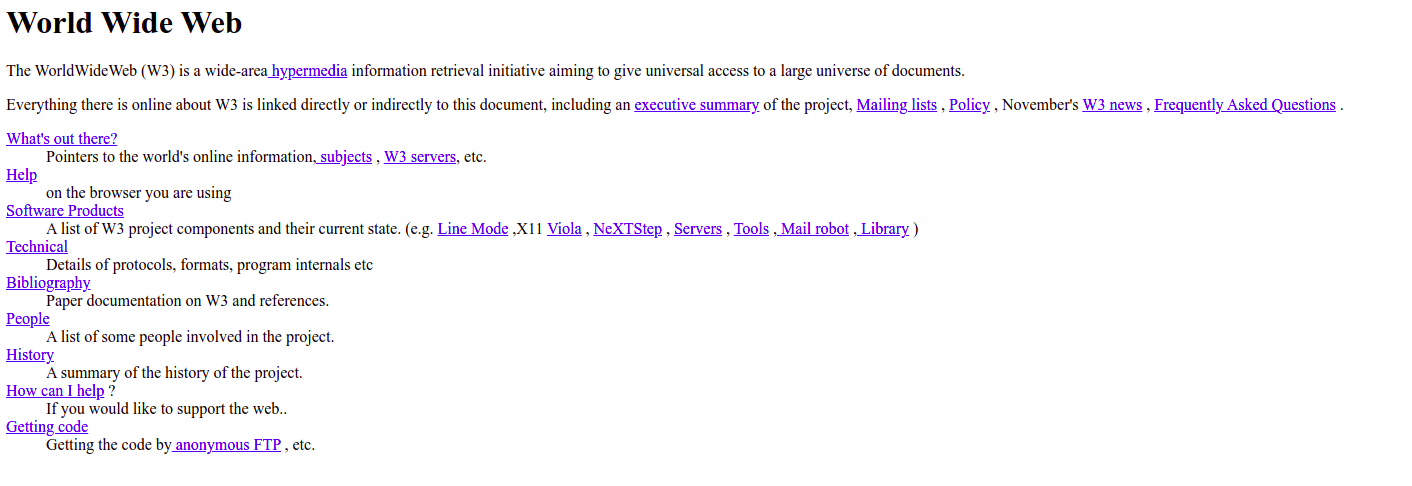
\includegraphics[width=16cm, keepaspectratio]{img/first_web_page.png}
    \caption{Primera página web}
    \label{fig:web}
\end{figure}

En la actualidad las principales ventajas de las tecnologías web son que se pueden utilizar en cualquier dispositivo, el usuario no necesita instalar nada más allá de un navegador web y su usabilidad es sencilla, pero dependen de Internet.\cite{juan}

Las páginas Web modernas utilizan el modelo Cliente-Servidor, en el que el cliente hace peticiones al servidor esperando una respuesta de este. Un mismo cliente puede estar conectado con varios servidores y a la vez interactúa con el usuario final normalmente a través de una interfaz gráfica. La parte del servidor se encarga de recibir las peticiones, analizarlas y procesarlas para enviar una respuesta. En las siguientes subsecciones, describimos algunas de las tecnologías más populares utilizadas en el desarrollo de páginas Web.

\begin{figure}[H]
    \centering
    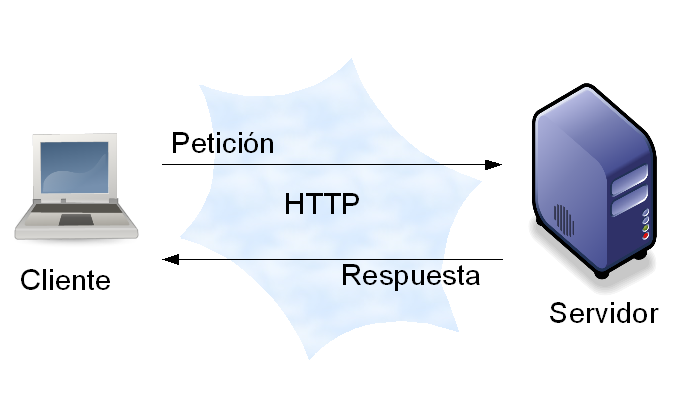
\includegraphics[width=10cm, keepaspectratio]{img/arquitectura.png}
    \caption{Arquitectura Cliente-Servidor}
    \label{fig:arquitectura}
\end{figure}

\subsection{Tecnologías web del lado del cliente}
Las tecnologías del lado del cliente suelen recibir el nombre de \textit{frontend}, son las que interactúan con el usuario, las más importantes son:

\begin{itemize}
  \item \textbf{HTML}:  Lenguaje de marcado que se encarga de dar la estructura a la página web. HTML utiliza etiquetas para mostrar los diferentes contenidos. La última versión es HTML5 donde se introducen las etiquetas de audio y vídeo.
  \item \textbf{CSS} \footnote{Cascading Style Sheets}: Lenguaje de estilo que se encarga del diseño de las páginas web. La última versión es CSS3
  \item \textbf{JavaScript}: Lenguaje de programación interpretado que permite la ejecución de código orientado a eventos (Por ejemplo, pulsar un botón). Puede actuar sobre el navegador a través de objetos integrados, es decir puede manipular el HTML.
\end{itemize}
\newpage
\subsection{Tecnologías web del lado del servidor}
Las tecnologías web del lado del servidor también llamadas \textit{backend} son las encargadas de procesar las peticiones del cliente y enviar una respuesta en forma de páginas HTML. Normalmente se utilizan \textit{frameworks }que son herramientas que te permiten desarrollar una aplicación web de forma ágil y sencilla a partir de librerías o funciones ya creadas. Algunos de estos \textit{frameworks} son:

\begin{itemize}
  \item \textbf{Django}: Está escrito en código Python. Django hace uso de plantillas permitiendo hacer páginas web más rápidas y sencillas. Gracias a su ORM \footnote{Object Relational Mapping
} no es necesario saberse el manejo de base de datos ya que este traduce directamente el código de Python.
  \item \textbf{Node.js}: Permite ejecutar código JavaScript fuera del navegador construido con el motor de JavaScript V8 de Chrome. Node.js utiliza un modelo de entrada y salida no bloqueante, no espera a que los procesos finalicen.
  \item \textbf{Symfony}: Utiliza de lenguaje de programación PHP \footnote{Hypertext Preprocessor}. Está basado en el patrón Modelo Vista Controlador (MVC). Symfony es muy flexible permitiéndote instalar únicamente lo que se necesite en vez del \textit{framework} completo.
  \item \textbf{Spring Boot}: Desarrollado para aplicaciones programadas en Java, surgió debido a que el Spring Framework era difícil de configurar. 
\item \textbf{Lavarel}: Framework de PHP. En comparación con otros \textit{frameworks }PHP su curva de aprendizaje es más baja. Es flexible y adaptable no solamente al MVC sino propone utilizar \textit{routes with clousures} a causa de lo cual reduce código.\cite{lavarel}
\end{itemize}

%%%%%%%%%%%%%%%%%%%%%%%%%
\section{Robótica Software }
La robótica es la ciencia o rama tecnológica encargada del estudio, diseño, creación y aplicación de los robots. En la actualidad existen muchas formas de estudiar robótica, puedes estudiarla tanto en universidades como en cursos.

Una parte de la robótica es la programación de estos robots por lo que se han buscado herramientas de aprendizaje sencillas y atrayentes para el usuario. En Internet se pueden encontrar diversas páginas web las cuales te enseñan sobre programación y robótica.

\begin{itemize}
\item \textbf{Snap!}\footnote{https://snap.berkeley.edu/}: Está basada en el código de programación de Scratch\footnote{ https://scratch.mit.edu/} , creada en la Universidad de Berkeley. Su código se basa en bloques permitiendo crear programas arrastrando y soltando para agrupar dichos bloques como un puzle. Esta aplicación la puedes utilizar tanto \textit{online} como descargándola y pudiendo utilizarla sin necesidad de Internet. La principal diferencia con Scratch es que te permite crear tus propios bloques utilizando JavaScript y así poder formar tu librería propia, también se puede crear listas avanzadas donde se puede almacenar cualquier tipo de dato incluso otras listas.  Esta aplicación web permite aprender a programar de una manera más visual y evitando los errores de sintaxis que se podrían cometer. Snap tiene una gran comunidad de usuarios que suben sus proyectos donde se puede aprender de ellos.\cite{app}
\end{itemize}

\begin{figure}[H]
    \centering
    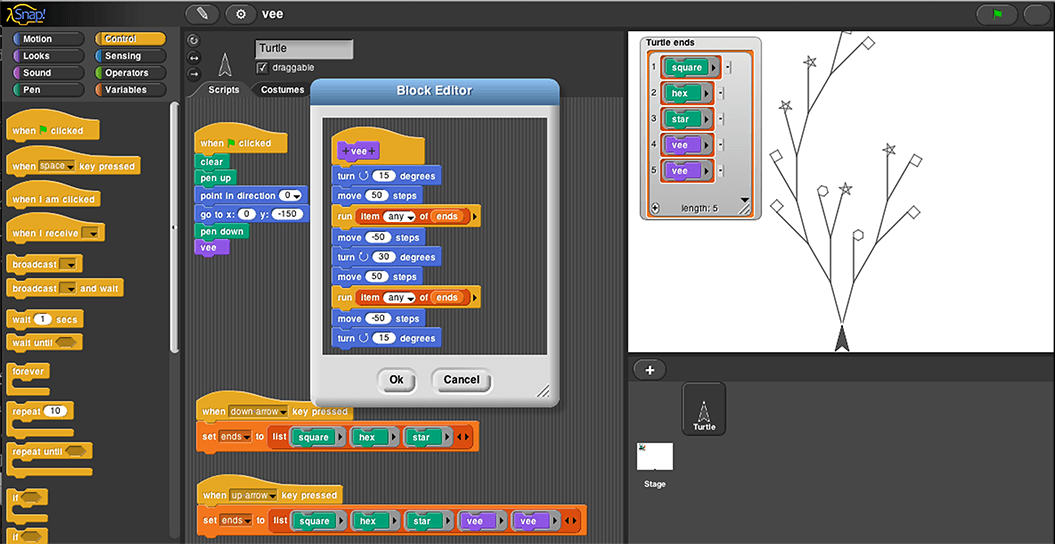
\includegraphics[width=15cm, keepaspectratio]{img/snap.png}
    \caption{Snap!}
    \label{fig:snap}
\end{figure}

\begin{itemize}
\item \textbf{Robocode}\footnote{https://robocode.sourceforge.io/}: Es un videojuego multiplataforma que consiste en la creación de un tanque robot el cual tendrá que atacar y esquivar otros tanques para no ser destruido. No es necesario descargar nada aparte de lo que viene en Robocode. Está dirigido para aprender Java y .NET. Nos podemos encontrar ligas donde las batallas de los robots transcurren en tiempo real, estas están divididas en diferentes categorías dependiendo del tamaño de código efectivo en bytes para que sean competiciones más justas. Se puede programar las tres partes del tanque que son: el cuerpo que se encarga de mover el tanque, el radar que detecta a los adversarios y el cañón que se utiliza para apuntar y disparar. La aplicación dispone de un editor de texto, un \textit{debugger} y un compilador, todos los robots que se vayan desarrollando se podrán guardar para futuras batallas.\cite{app}
\end{itemize}

\begin{figure}[H]
    \centering
    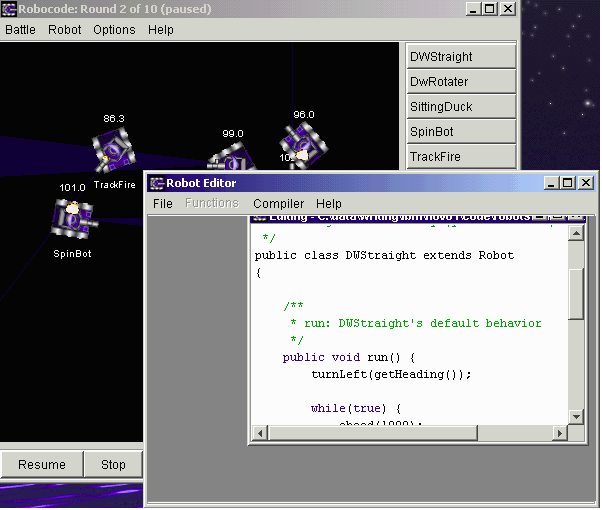
\includegraphics[width=10cm, keepaspectratio]{img/Robocode.png}
    \caption{Robocode}
    \label{fig:robocode}
\end{figure}

\begin{itemize}
\item \textbf{CodeCombat}\footnote{ https://codecombat.com/} Es una página web donde a través de un personaje se enseña a programar en diferentes lenguajes como Python, JavaScript, C++, entre otros. El objetivo del juego es ir superando los diferentes niveles, los cuales van aumentando de dificultad. Esta compuesto por 110 niveles gratuitos con opción de jugar más niveles si se paga, además pagando se pueden desbloquear diferentes héroes, aprender a programar juegos y páginas web.\cite{app}
\end{itemize}

\begin{figure}[H]
    \centering
    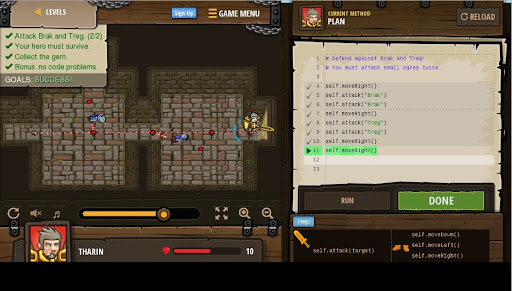
\includegraphics[width=15cm, keepaspectratio]{img/Codecombat.jpg}
    \caption{CodeCombat}
    \label{fig:codecombat}
\end{figure}

\section{Unibotics 1.0}

Página web donde se desarrolla este Trabajo de Fin  de Grado en la cual se enseña a programar de una manera llamativa y divertida para estudiantes universitarios, en concreto para aprender a programar sobre robótica. La página consta de cuatro ejercicios, el primero llamado \textit{follow line} consiste en programar un coche de fórmula uno para que realice el circuito siguiendo una linea roja, en el segundo ejercicio, \textit{Obstacle avoidance}, se deberá programar un coche de fórmula uno para que haga el circuito evitando otros coches para ello se utilizará el algoritmo de navegación VFF\footnote{Virtual Force Field} que consiste en que los objetos que se tienen que esquivar generan una fuerza repulsiva al coche de formula uno mientras que el destino genera una fuerza atrayente, el siguiente ejercicio es \textit{Vacuum cleaner} en el cual hay que programar una aspiradora para que pase por toda la superficie de una casa y el último ejercicio \textit{Localized Vacuum Cleaner} tiene como objetivo el mismo que \textit{Vacuum Cleaner} pero en este caso la aspiradora sabe su ubicación.\\

\newpage
Se puede programar los ejercicios directamente desde la web sin la necesidad de instalar la aplicación, en ellos puedes subir o guardar el código realizado, además hay un evaluador automático de estilo. Se utiliza el lenguaje Python para poder realizar los ejercicios. Unibotics utiliza una imagen de docker llamada RADI \footnote{https://hub.docker.com/r/jderobot/robotics-academy/}(\textit{Robots Academy Docker Image} donde están preinstaladas las dependencias y así no se tiene que descargar nada localmente, además esta basada en ROS\footnote{https://www.ros.org/} ( \textit{framework} flexible para escribir \textit{software} de robots) y Gazebo9\footnote{http://gazebosim.org/} (Simulador de robots).\cite{robotics}\\

Actualmente se han añadido numerosas mejoras y más ejercicios a parte de lo implementado para la realización de este TFG.

\begin{figure}[H]
    \centering
    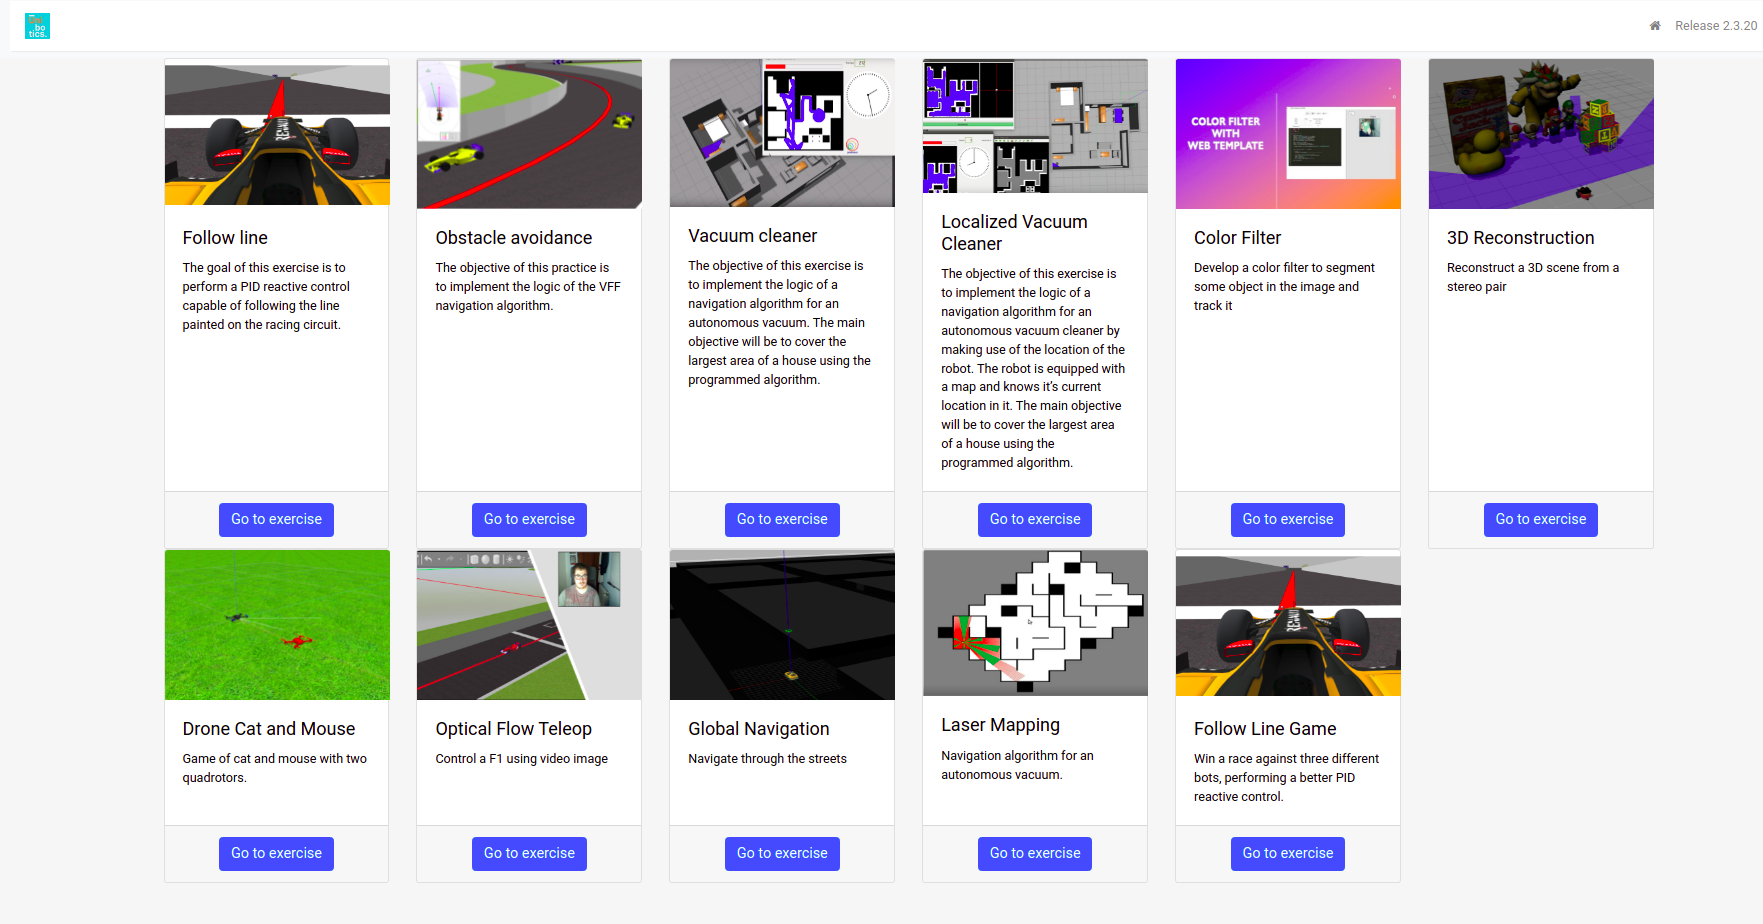
\includegraphics[width=15cm, keepaspectratio]{img/unibotics.png}
    \caption{Unibotics en la actualidad}
    \label{fig:unibotics}
\end{figure}

\newpage
\section{Estructura del documento}

Este Trabajo de Fin de Grado consta de de los siguientes capítulos:

\begin{itemize}
    \item \textit{Capítulo 1 Introducción}: introducción a las tecnologías web, a páginas web educativas sobre robótica y Unibotics antes de la realización de este TFG.
    \item \textit{Capítulo 2 Objetivos y Metodología}: Descripción de los diferentes objetivos a cumplir en el TFG y la metodología seguida para la realización de estos.
    \item \textit{Capítulo 3 Herramientas utilizadas}: se describen las diferentes tecnologías web utilizadas en este trabajo y las herramientas usadas para la recogida y grabación de datos y la visualización de estadísticas automáticas.
   \item \textit{Capítulo 4 Analíticas de Elasticsearch y Dash}: en este capítulo se expone el diseño y la implementación de la recogida de sondas y su posterior visualización en la plataforma de Unibotics.
  \item \textit{Capítulo 5 Conclusiones}: se desarrollan las conclusiones de los resultados obtenidos en este TFG, además de las competencias que se ha adquirido y futuros trabajos que se podrían realizar a partir de este.
   \end{itemize}